\section{Trajectory Planning - Laparoscopic tool manipulation}

\begin{frame}
\frametitle{Tool pose}

\begin{columns}
\column{0.4\textwidth}
\begin{center}
\begin{figure}[!htb]
\centering
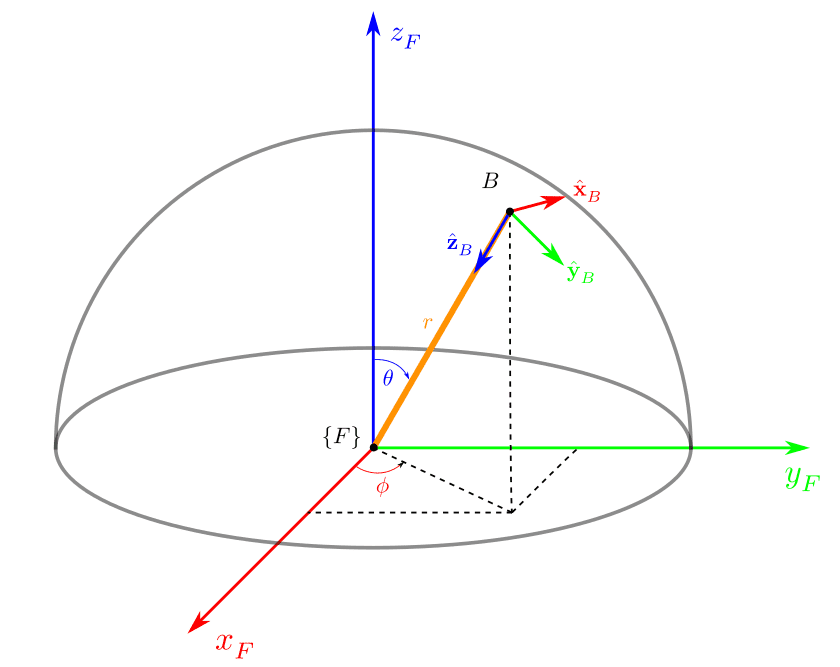
\includegraphics[width=\textwidth]{../images/fulcrum-space.png}\\
\end{figure}
\end{center}
\[
{}^{F}T_B = \begin{bmatrix}
{}^{F}R_B & {}^{F}\mathbf{p}^{}_B \\
\mathbf{0} & 1 \\
\end{bmatrix}
\]
where
\[
{}^{F}R_B = \begin{bmatrix}
\hat{\mathbf{x}}^{}_B & \hat{\mathbf{y}}^{}_B & \hat{\mathbf{z}}^{}_B \\
\end{bmatrix}
\]

\column{0.5\textwidth}
Calculate orientation vectors using spherical coordinate unit vectors
\[
\hat{\mathbf{x}}^{}_B = \hat{\mathbf{\phi}}
= \begin{bmatrix}
-\sin(φ) \\
\cos(φ) \\
0 \\
\end{bmatrix}
\]

\[
\hat{\mathbf{y}}^{}_B = \hat{\mathbf{\theta}}
= \begin{bmatrix}
\cos(θ)\cos(φ) \\
\cos(θ)\sin(φ) \\
- \sin(θ) \\
\end{bmatrix}
\]

\[
\hat{\mathbf{z}}^{}_B = \hat{\mathbf{r}}
= \begin{bmatrix}
\sin(θ)\cos(φ) \\
\sin(θ)\sin(φ) \\
\cos(θ) \\
\end{bmatrix}
\]

\end{columns}
\end{frame}

\begin{frame}
\frametitle{The Fulcrum Effect}
\begin{center}
\begin{figure}[!htb]
\centering
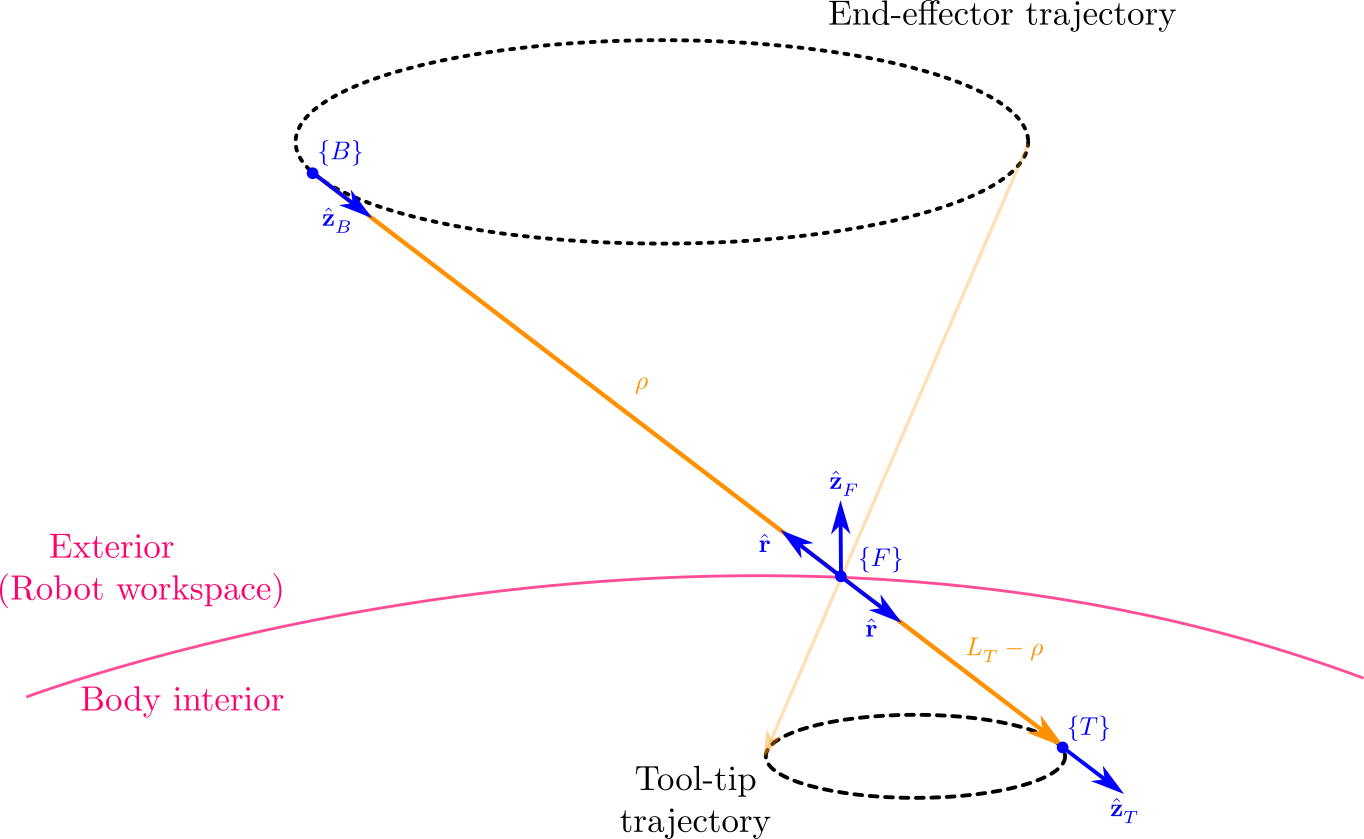
\includegraphics[width=0.9\textwidth]{../images/circular-trajectory-wrt-fulcrum.png}\\
\end{figure}
\end{center}
\end{frame}

\subsection{Trajectory planning in cartesian coordinates}

\begin{frame}
\frametitle{Line segment trajectory of tool tip}

\begin{columns}
\column{0.6\textwidth}
\begin{center}
\begin{figure}[!htb]
\centering
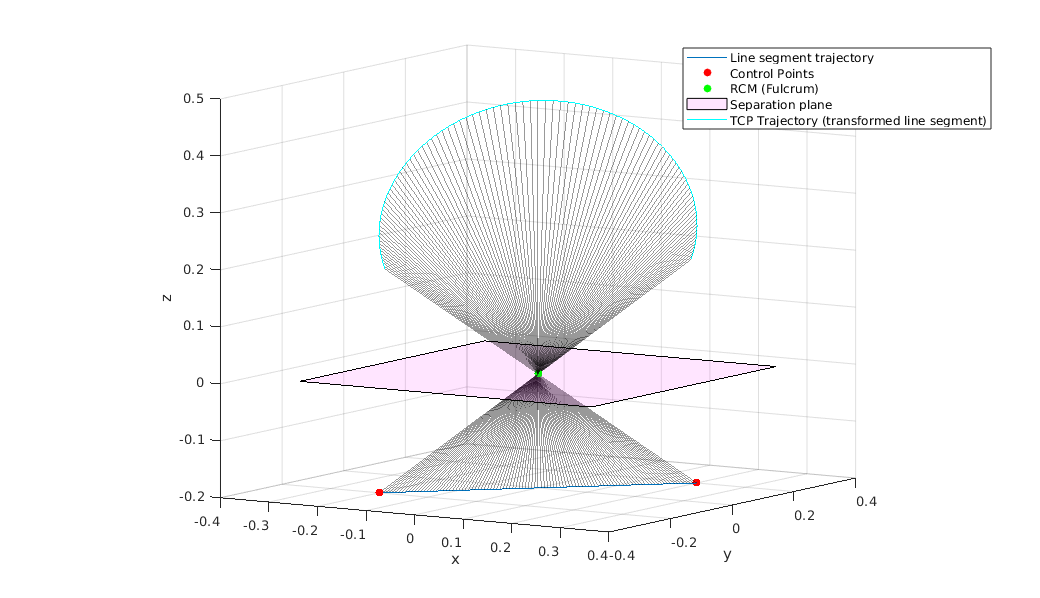
\includegraphics[width=\textwidth]{../images/rcm_trajectories/rcm_lineseg_traj.png}\\
\caption{A Line segment trajectory and it's transformation due to the Fulcrum Effect}
\end{figure}
\end{center}

\column{0.4\textwidth}
\begin{center}
\begin{figure}[!htb]
\centering
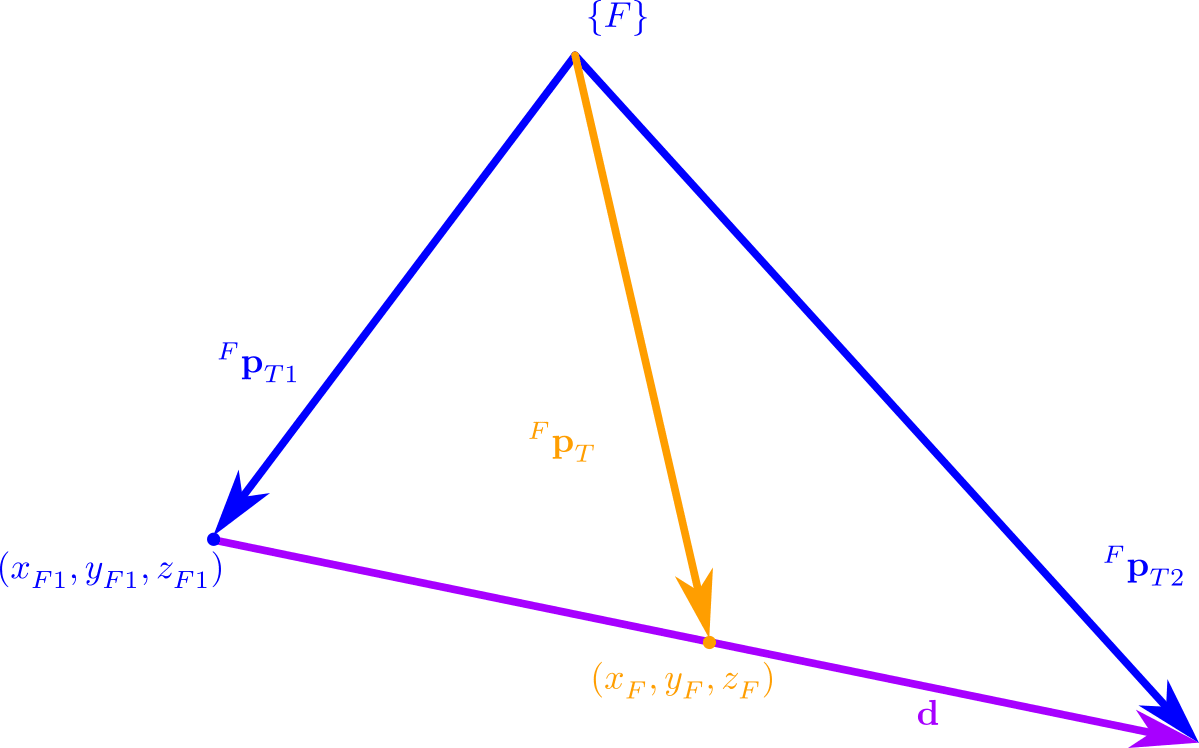
\includegraphics[width=\textwidth]{../images/line-segment-trajectory-wrt-fulcrum.png}\\
\end{figure}
\end{center}
\[
\begin{cases}
x^{}_{F} = (1-s)x^{}_{F1} + sx^{}_{F2} \\
y^{}_{F} = (1-s)y^{}_{F1} + sy^{}_{F2} \\
z^{}_{F} = (1-s)z^{}_{F1} + sz^{}_{F2}
\end{cases}
\]

\end{columns}
\end{frame}


\begin{frame}
\frametitle{Circular trajectory of tool tip}

\begin{columns}
\column{0.6\textwidth}
\begin{center}
\begin{figure}[!htb]
\centering
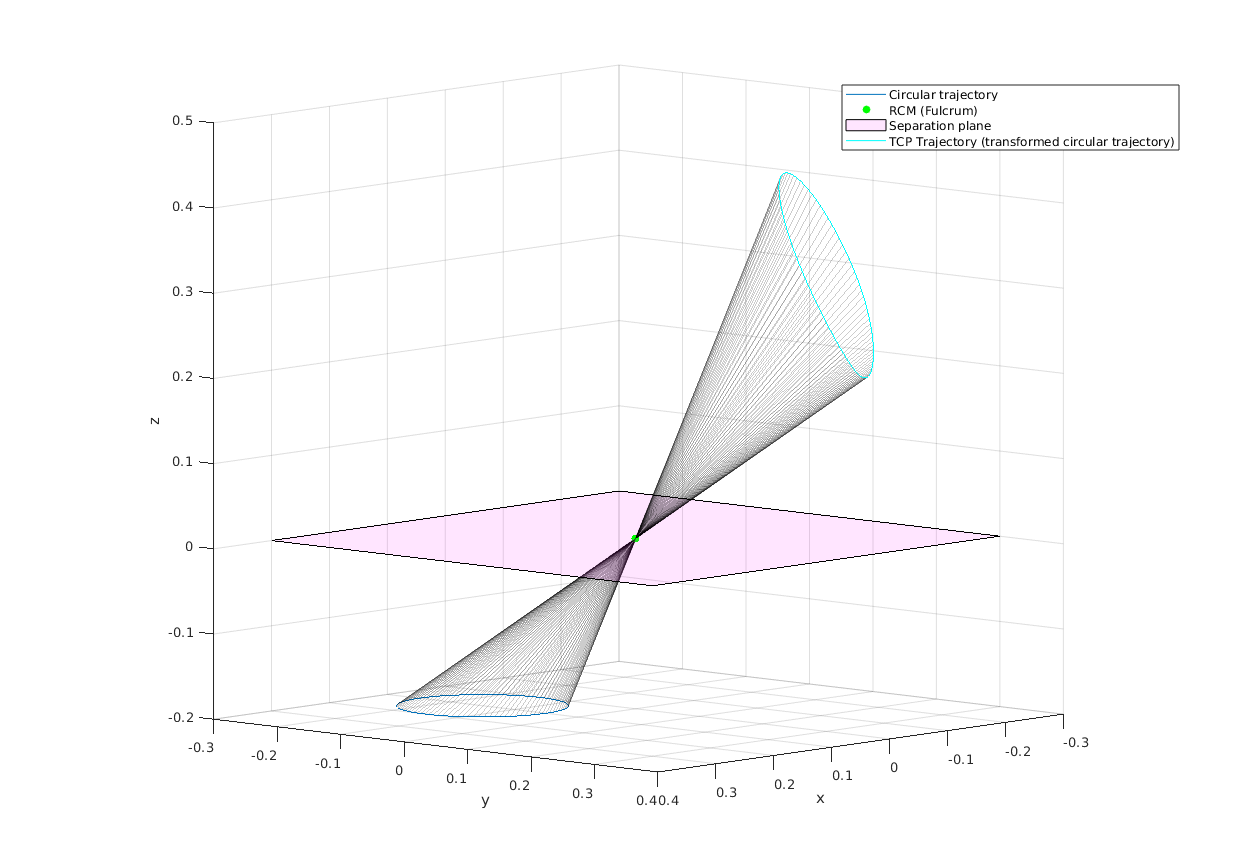
\includegraphics[width=\textwidth]{../images/rcm_trajectories/rcm_circle_traj.png}\\
\caption{Circular trajectory of tool tip with respect to Fulcrum reference frame and it's transformation via the Fulcrum Effect}
\end{figure}
\end{center}

\column{0.4\textwidth}
\[
\begin{cases}
x^{}_{F} = r_0\cos(2πs) + x^{}_{F0} \\
y^{}_{F} = r_0\sin(2πs) + y^{}_{F0} \\
z^{}_{F} = z^{}_{F0}
\end{cases} ,
\]
\[
s \in [0, 1]
\]

\[
\begin{cases}
r = \sqrt{x^{2}_{F} + y^{2}_{F} + z^{2}_{F}} \\
θ = atan2 \left( \sqrt{x^{2}_{F} + y^{2}_{F}}, z^{}_{F} \right) \\
φ = atan2(y^{}_{F}, x^{}_{F})
\end{cases}
\]
\end{columns}
\end{frame}

\begin{frame}
\frametitle{Circular trajectory of tool tip}

\begin{columns}
\column{0.5\textwidth}
\begin{center}
\begin{figure}[!htb]
\centering
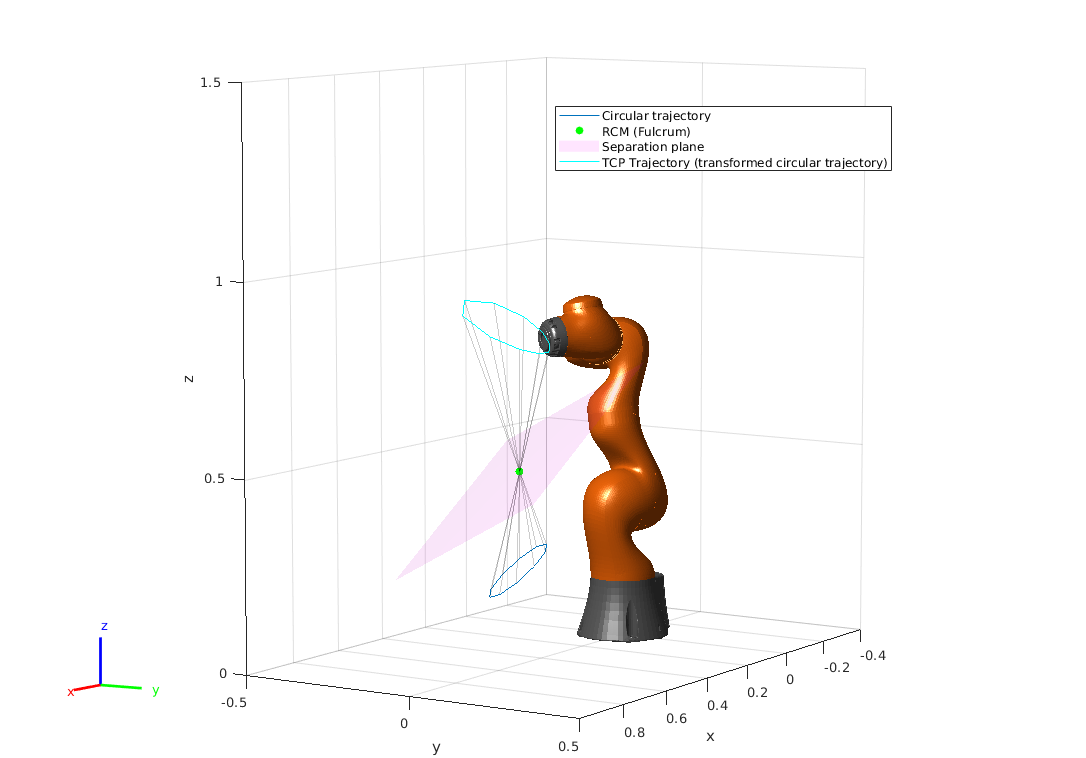
\includegraphics[width=\textwidth]{../images/rcm_trajectories/robot-pose-random-rcm-circle-traj.png}\\
\caption{Circular trajectory that lies on an a plane of arbitrary orientation with respect to the fulcrum point}
\end{figure}
\end{center}

\column{0.5\textwidth}
\begin{center}
\begin{figure}[!htb]
\centering
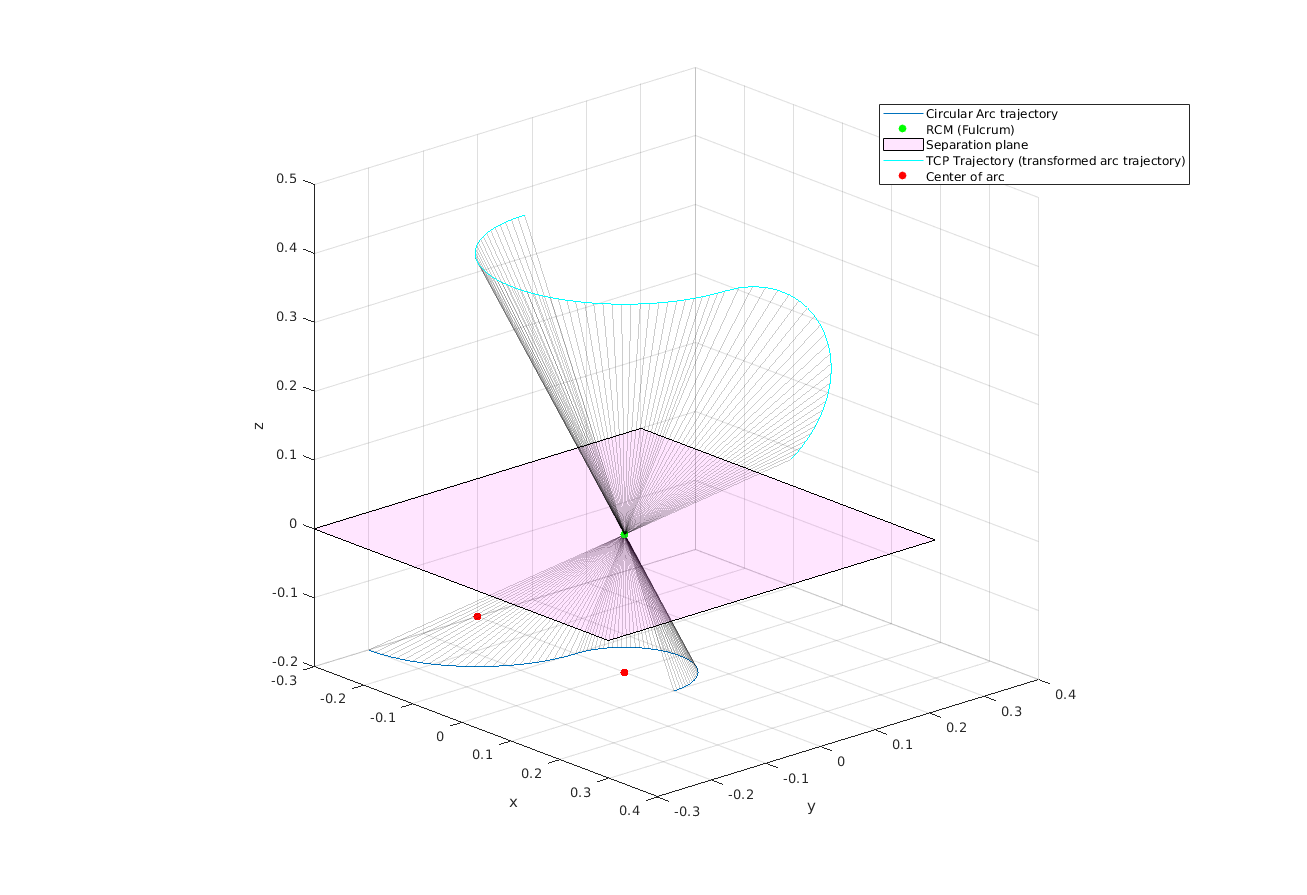
\includegraphics[width=\textwidth]{../images/rcm_trajectories/rcm_arcs_traj.png}\\
\caption{Circular arc trajectory of tool tip with respect to Fulcrum reference frame and it's transformation via the Fulcrum Effect. In this trajectory 2 circular arcs are used}
\end{figure}
\end{center}
\end{columns}
\end{frame}


\begin{frame}
\frametitle{Helical trajectory of tool tip}

\begin{columns}
\column{0.6\textwidth}
\begin{center}
\begin{figure}[!htb]
\centering
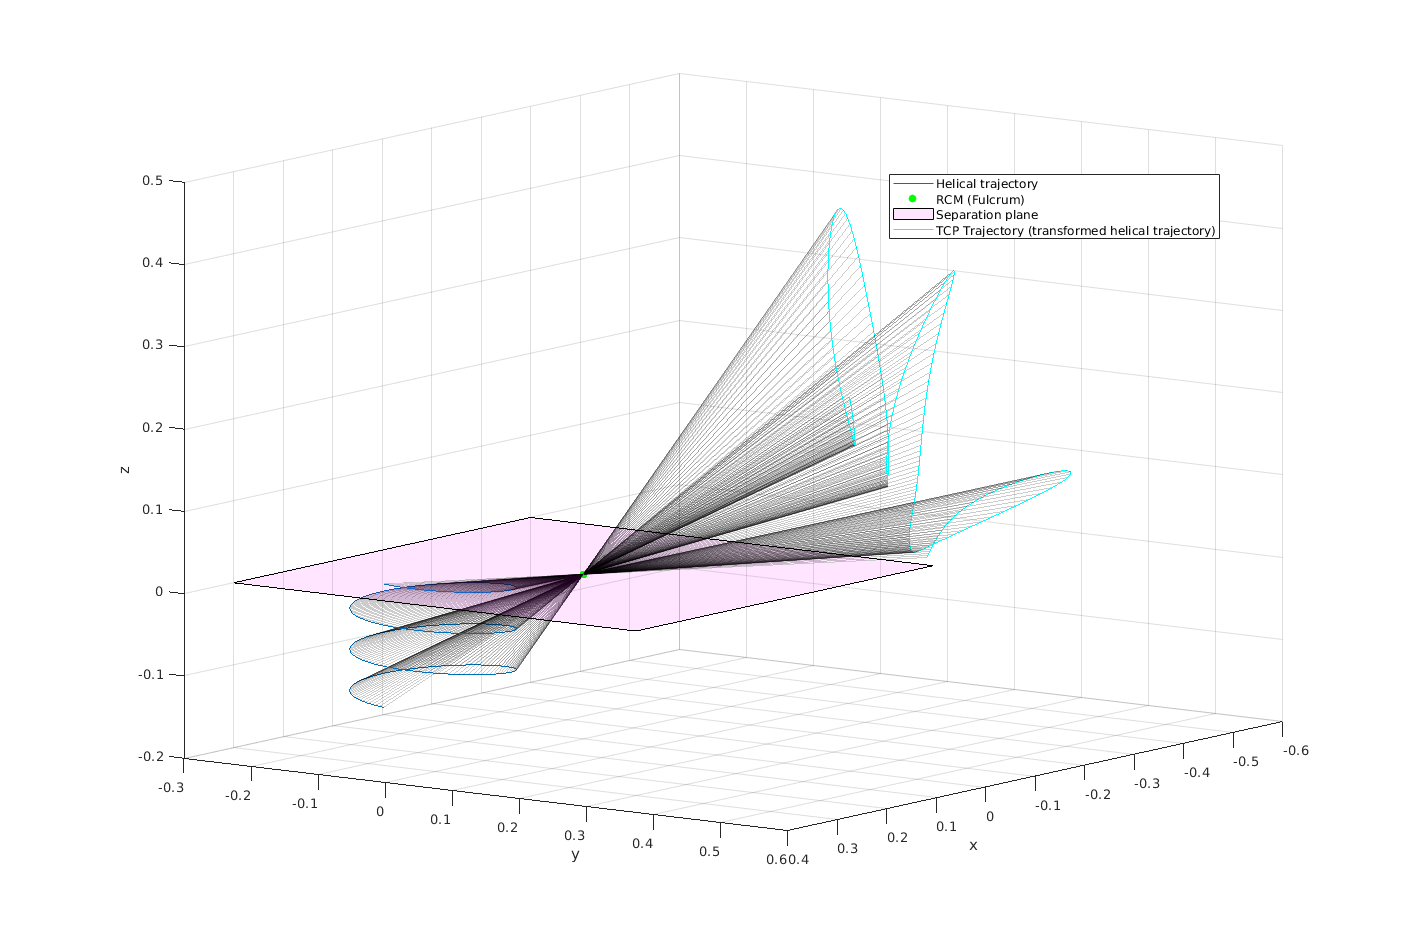
\includegraphics[width=\textwidth]{../images/rcm_trajectories/rcm_helical_traj.png}\\
\caption{Helical trajectory of tool tip with respect to Fulcrum reference frame and it's transformation via the Fulcrum Effect}
\end{figure}
\end{center}

\column{0.4\textwidth}
\[
\begin{cases}
x^{}_{F} = r_0\cos(2πs) + x^{}_{F0} \\
y^{}_{F} = r_0\sin(2πs) + y^{}_{F0} \\
z^{}_{F} = \pm βs
\end{cases}
\]
\begin{center}
\[
s \in \left[ 0, τ \right]
\]
$τ$: cycles\\
$β/r_0$: slope (aka pitch)
\end{center}
\end{columns}
\end{frame}


\begin{frame}
\frametitle{Cubic Spline trajectory of tool tip}

\begin{columns}
\column{0.5\textwidth}
\begin{align*}
x_i(s) = & a_i(s-s_i)^3 + b_i(s-s_i)^2 + \\ &+ c_i(s-s_i) + d_i
\end{align*}
\[
s_i \leqslant s \leqslant s_{i+1}
\]
boundary conditions $\Rightarrow α_i,b_i,c_i,d_i \in \mathbb{R}$
\[
x_i(s_i) = x_i
\]
\[
x_i(s_{i+1}) = x_{i+1}
\]
\[
\dot{x}_i(s_i) = \dot{x}_i
\]
\[
\dot{x}_i(s_{i+1}) = \dot{x}_{i+1}
\]

\column{0.5\textwidth}
\begin{center}
\begin{figure}[!htb]
\centering
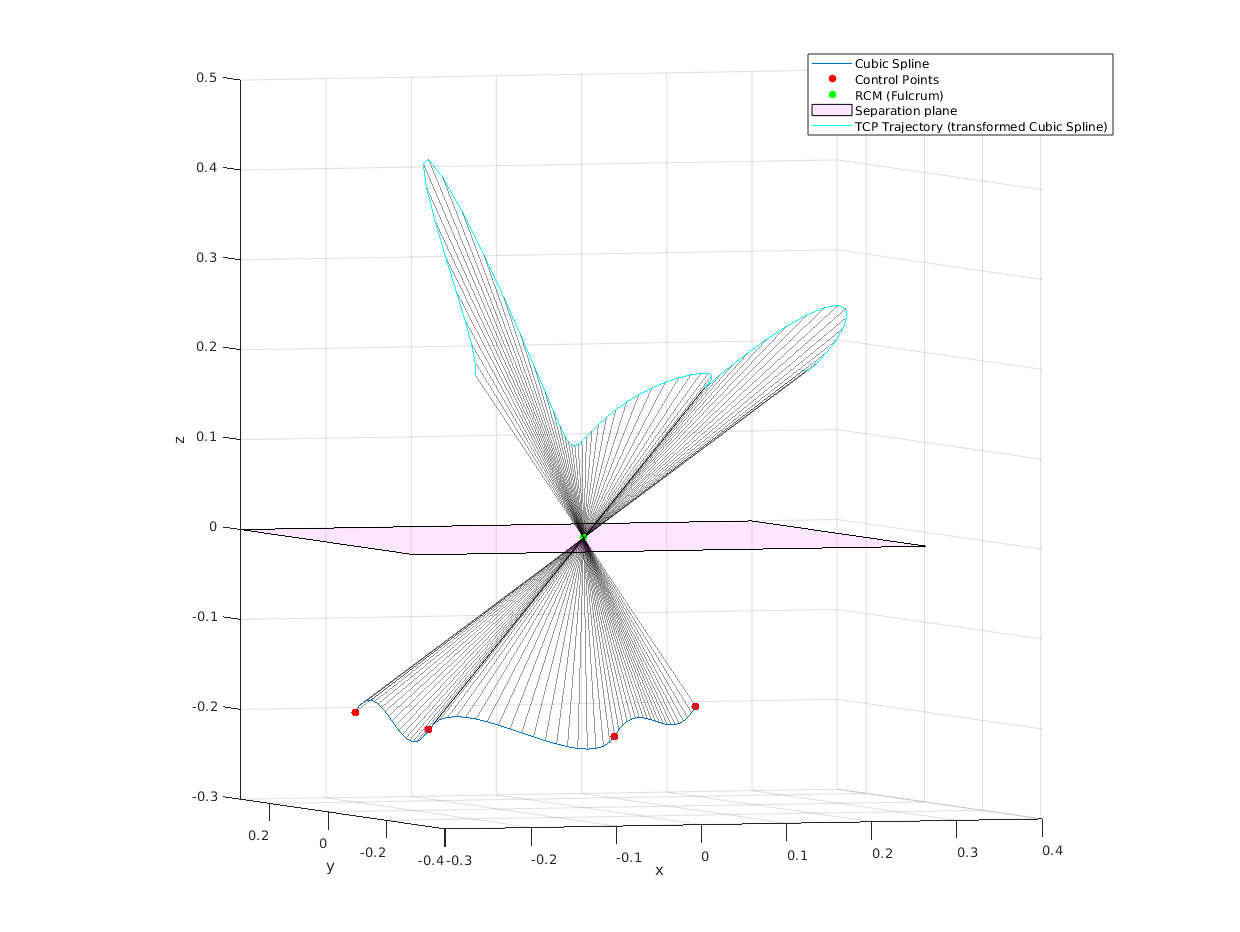
\includegraphics[width=\textwidth]{../images/rcm_trajectories/rcm_cubic_traj.png}\\
\caption{A Cubic Spline trajectory and it's transformation via the Fulcrum Effect}
\end{figure}
\end{center}
\end{columns}
\end{frame}

\begin{frame}
\frametitle{B-Spline trajectory of tool tip}
\begin{columns}
\column{0.4\textwidth}
\begin{center}
\begin{figure}[!htb]
\centering
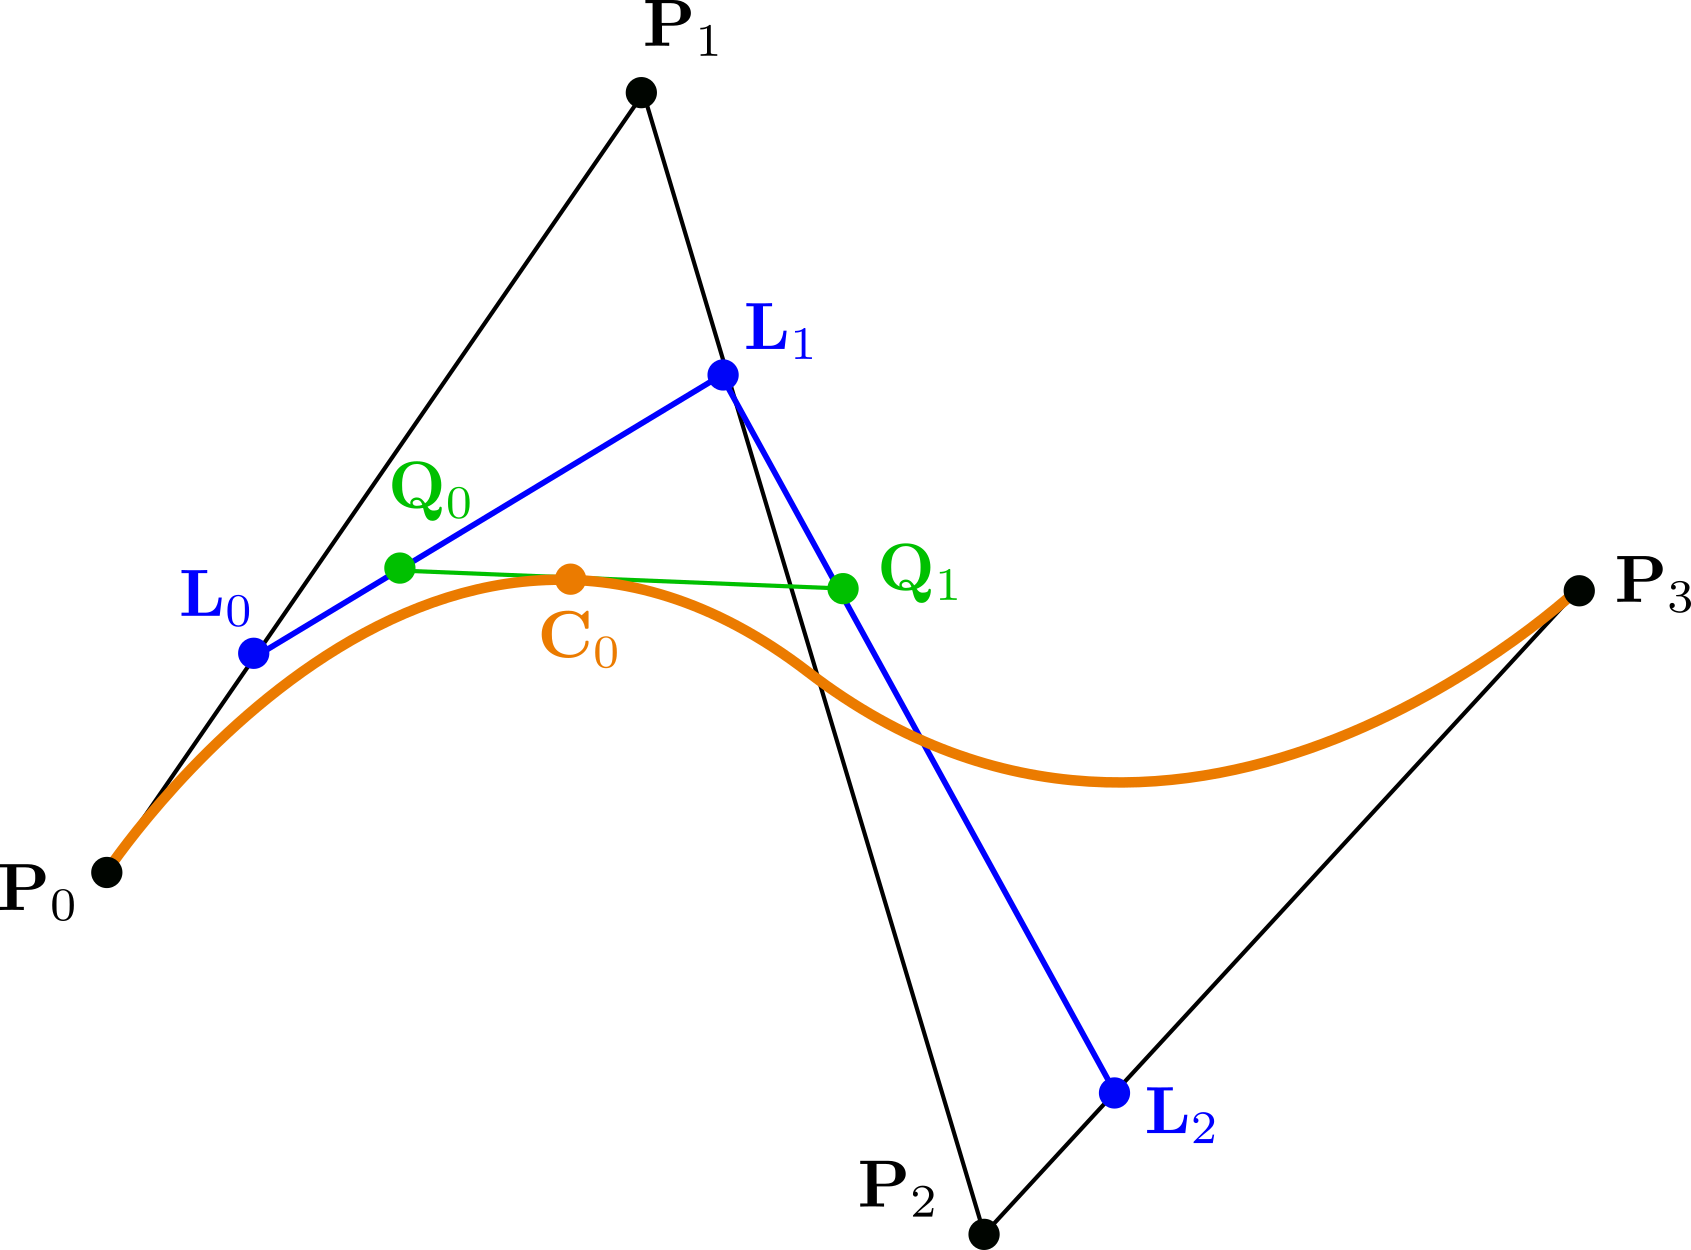
\includegraphics[width=\textwidth]{../images/bezier-curve.png}\\
\caption{Cubic B\'ezier curve calculated using cubic interpolation of 4 control points} 
\end{figure}
\end{center}

\column{0.6\textwidth}
\[
\mathbf{L}_0(s) = (1-s)\mathbf{P}_0 + s\mathbf{P}_1
\]
\[
\mathbf{Q}_0(s) = (1-s)\mathbf{L}_0(s) + s\mathbf{L}_1(s)
\]
\[
\mathbf{C}_0(s) = (1-s)\mathbf{Q}_0(s) + s\mathbf{Q}_1(s)
\]
\begin{align*}
    \mathbf{C}_0(s) = (1-s)^3\mathbf{P}_0 &+ 3(1-s)^2 s\mathbf{P}_1 + \\ &+ 3(1-s)s^2\mathbf{P}_2 + s^3\mathbf{P}_3
\end{align*}
\end{columns}
\end{frame}

\begin{frame}
\frametitle{B-Spline trajectory of tool tip}
\begin{columns}
\column{0.6\textwidth}
\begin{center}
\begin{figure}[!htb]
\centering
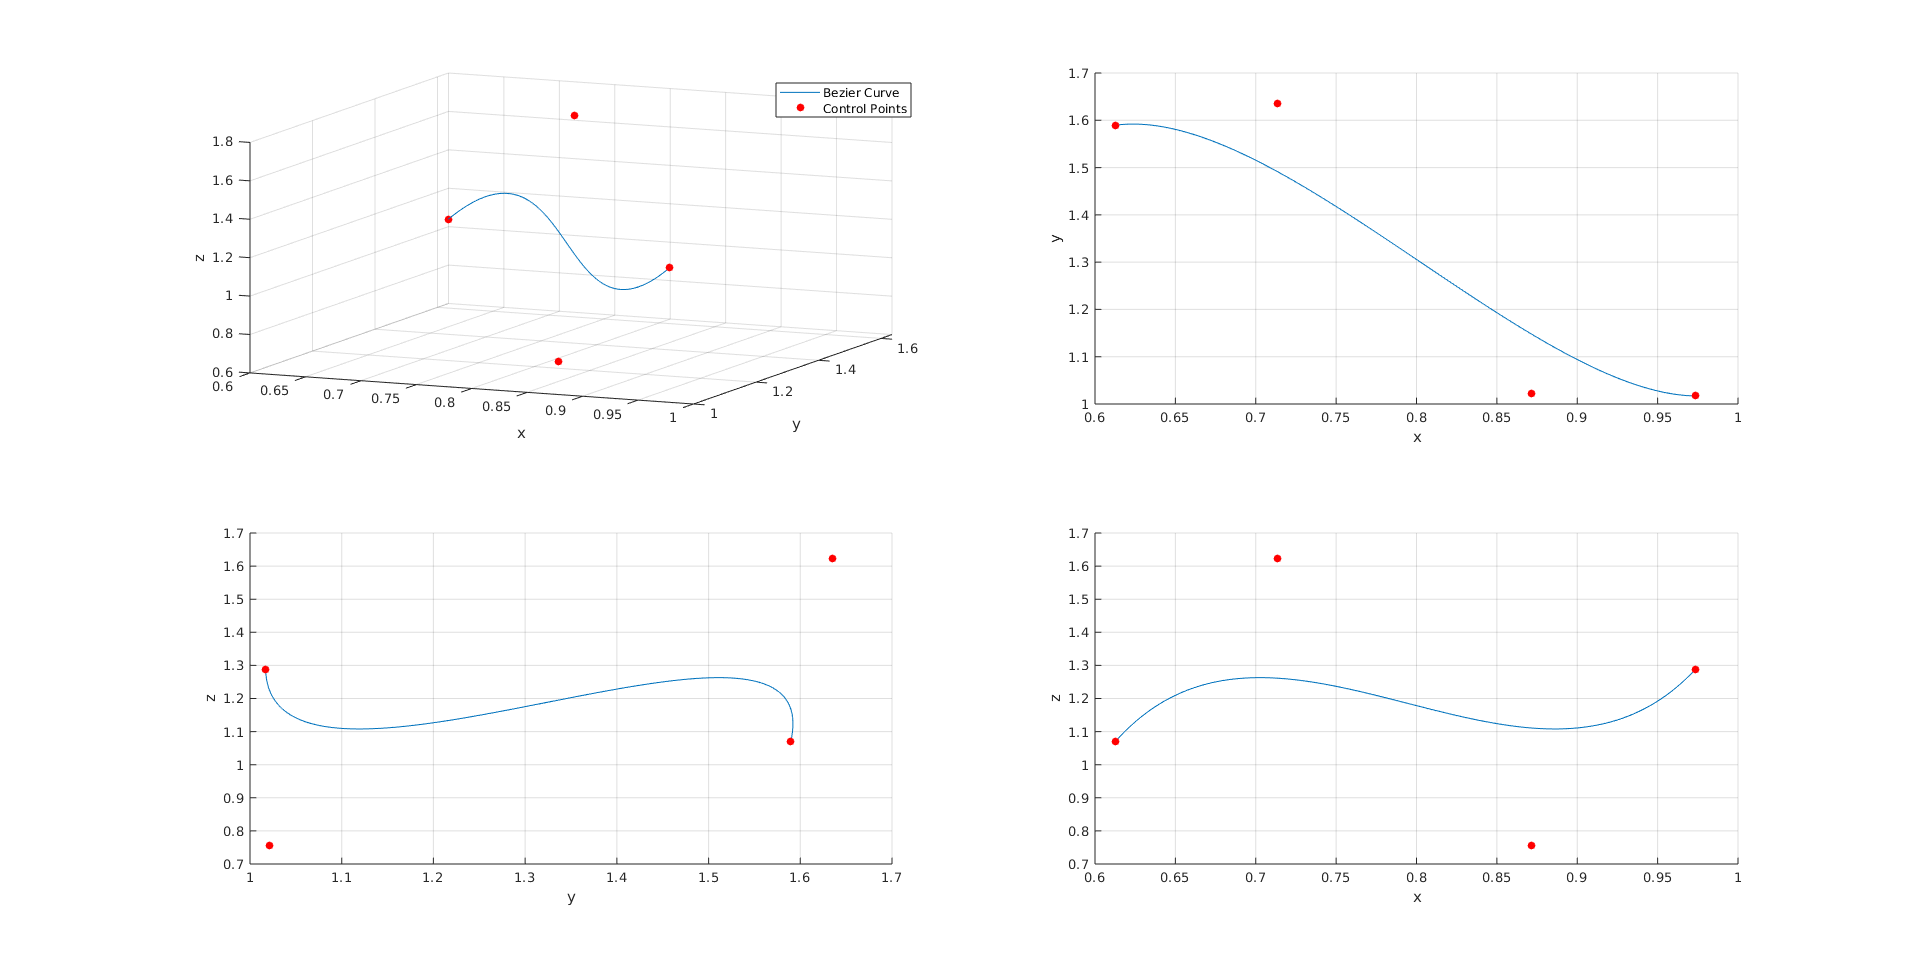
\includegraphics[width=\textwidth]{../images/bezier_path.png}\\
\caption{A cubic B\'ezier curve calculated and plotted in MATLAB} 
\end{figure}
\end{center}

\column{0.4\textwidth}
\begin{center}
\begin{figure}[!htb]
\centering
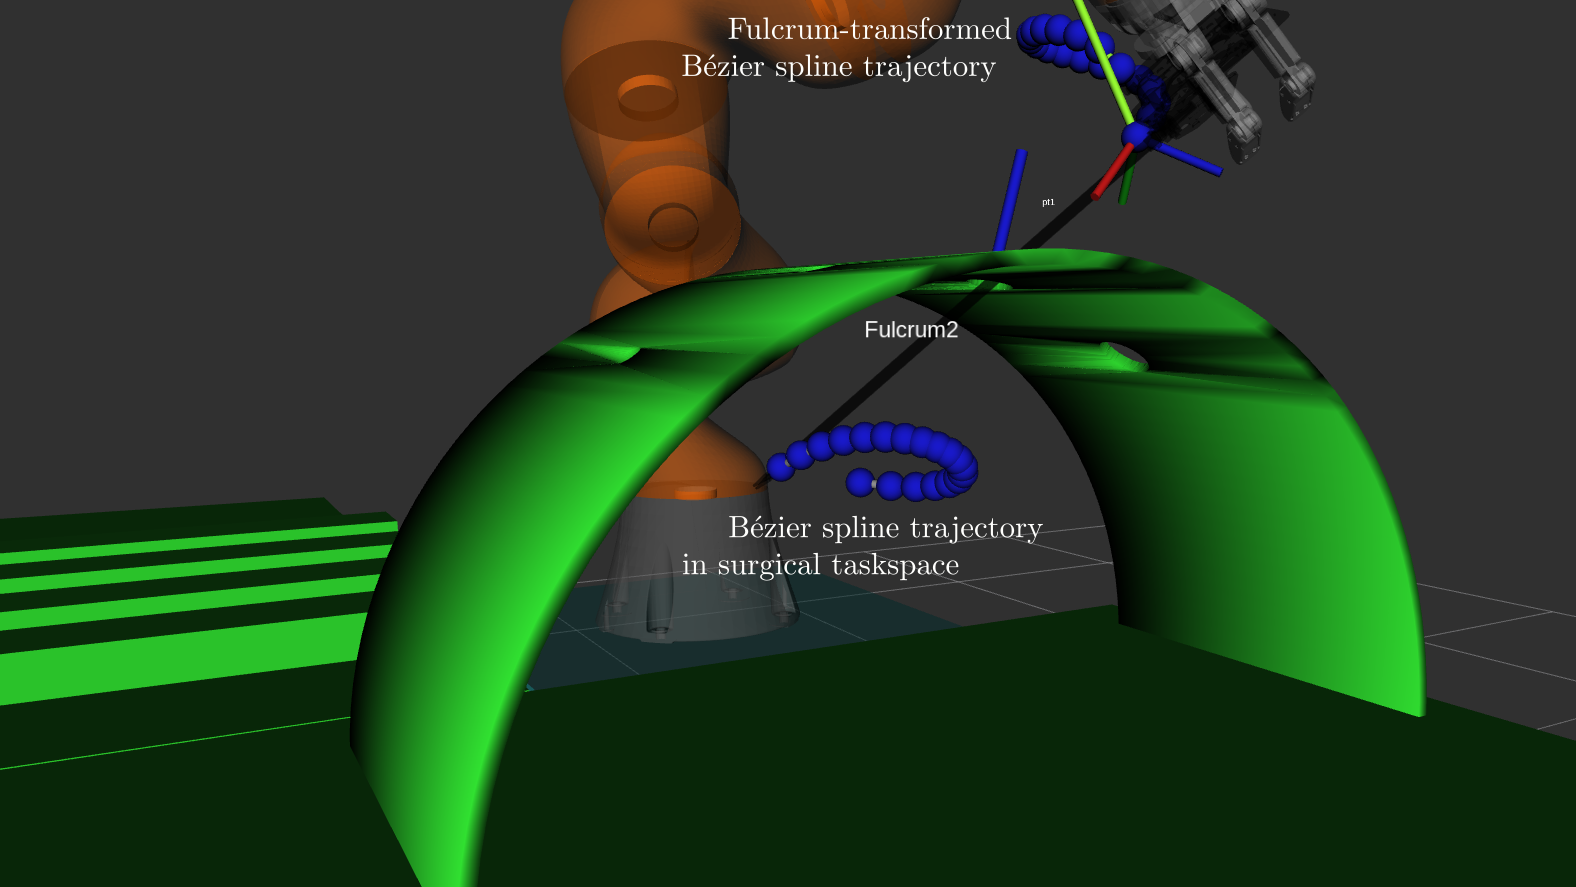
\includegraphics[width=\textwidth]{../images/robot_planner3/3d_bezier_spline.png}
\caption{Experiment 3d: Create the B-spline trajectory inside the surgical site (below the green mounting dock) and transform it via the fulcrum transformation to a trajectory for the robot's TCP.}
\label{robot-planner3d-bezier-spline}
\end{figure}
\end{center}

\end{columns}
\end{frame}


\subsection{Trajectory planning in joints' space}

\begin{frame}
\frametitle{Trajectory planning in joints' space}
\begin{columns}
\column{0.32\textwidth}
\begin{center}
\begin{figure}[H]
\centering
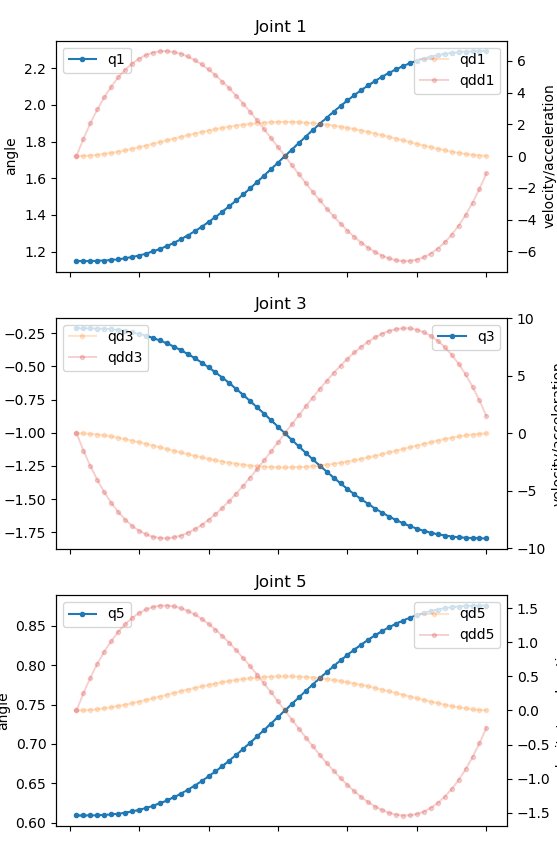
\includegraphics[width=\textwidth]{../images/robot_planner3/3e_joint_polynomial_half.png}
\caption{Quintic polynomial trajectories}
\end{figure}
\end{center}

\column{0.32\textwidth}
\begin{center}
\begin{figure}[H]
\centering
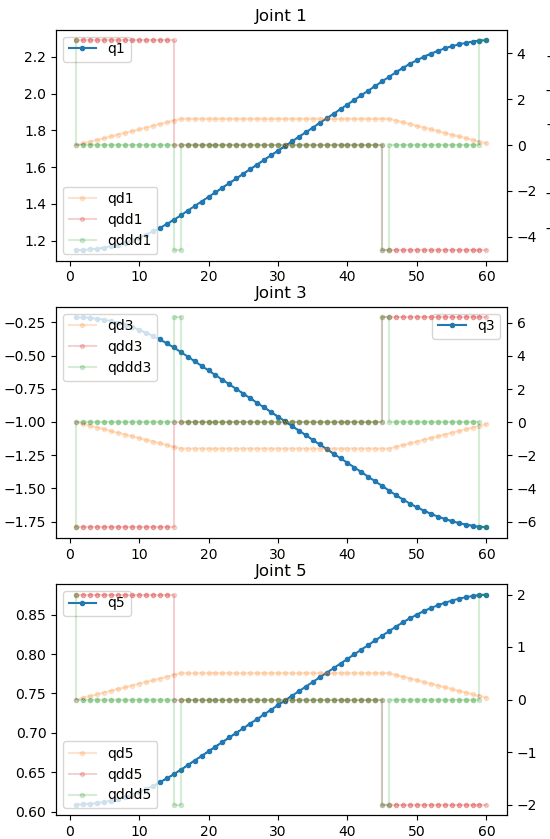
\includegraphics[width=\textwidth]{../images/robot_planner3/3f_trapezoid1_half.png}
\caption{Trajectories with trapezoid velocity profile}
\end{figure}
\end{center}

\column{0.32\textwidth}
\begin{center}
\begin{figure}[H]
\centering
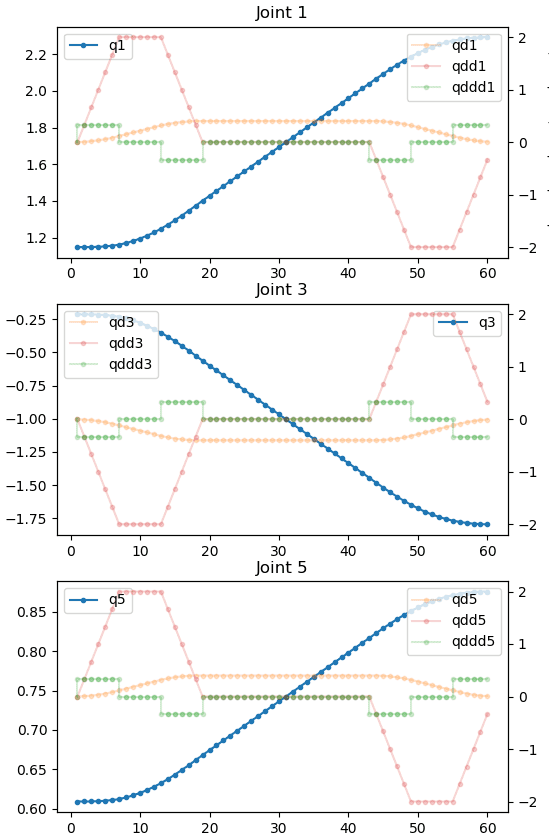
\includegraphics[width=\textwidth]{../images/robot_planner3/3g_s_curve_half.png}
\caption{Trajectories with s-curve velocity profile}
\end{figure}
\end{center}
\end{columns}
\end{frame}
